  \documentclass[letter]{article}
\usepackage[utf8]{inputenc}
\usepackage[margin=1in]{geometry}
\usepackage{tikz}
\usepackage{ulem}
\usepackage{graphics}
\usepackage{sidecap}
\usepackage{wrapfig}
\usepackage[toc,page]{appendix}

\usepackage{hyperref}
\usepackage{parskip}

\hypersetup{
    colorlinks,%
    citecolor=black,%
    filecolor=black,%
    linkcolor=black,%
    urlcolor=black
}

\def\dashuline{\bgroup 
  \ifdim\ULdepth=\maxdimen  % Set depth based on font, if not set already
	  \settodepth\ULdepth{(j}\advance\ULdepth.4pt\fi
  \markoverwith{\kern.15em
	\vtop{\kern\ULdepth \hrule width .3em}%
	\kern.15em}\ULon}

\newcounter{foot}
\setcounter{foot}{1}

\setlength\parindent{2em}

\author{John Muir Institute of the Environment}
\date{\today}
\title{QRAAT}
	
\begin{document}
\maketitle

\begin{abstract}
This could eventually be our doc for QRAAT. For now, this just outlines configuration 
stuff for the prototype system. Build this doc with pdflatex (sudo apt-get install pdflatex). 
\end{abstract}

\tableofcontents
\pagebreak

\section{Overview} 
\subsection{Hardware}

Along with the antenna, preamps, RMG receiver, batteries, and solar panels, a node 
in the QRAAT network consists of a router to the network, a field computer, and a network-addressible 
powerswitch. The last two are pictured together with the receiver in Figure 1. 

\textbf{Field computer}. To run the software defined radio remotely, we require a headless system
that can run on limited power and be able to withstand high temperatures. The ideal system would 
have no moving parts---fanless, solid-state memory instead of a harddrive---and draw only a few 
amps. However, in our tests with various solutions, we've concluded that a dual-core CPU is 
required at a minimum.\footnote{One solution we tried was the net6501-70 from Soekris Engineering, which
ships with a single 1.6 Ghz Atom core. The backend software was installed on top of the OpenWRT operating 
system, a stripped-down version of GNU/Linux meant for embedded systems. The Soekris board failed to 
process the radio signal at line-rate with the system running full-bore.} The parallelisation that 
can be achieved with multiple cores drastically improves the performance of the signal processing
software. There are a number of products available that strike a comprimise between power consumption 
\begin{wrapfigure}{h}{0.5\textwidth}
  \vspace{-10pt}
  \begin{center}
    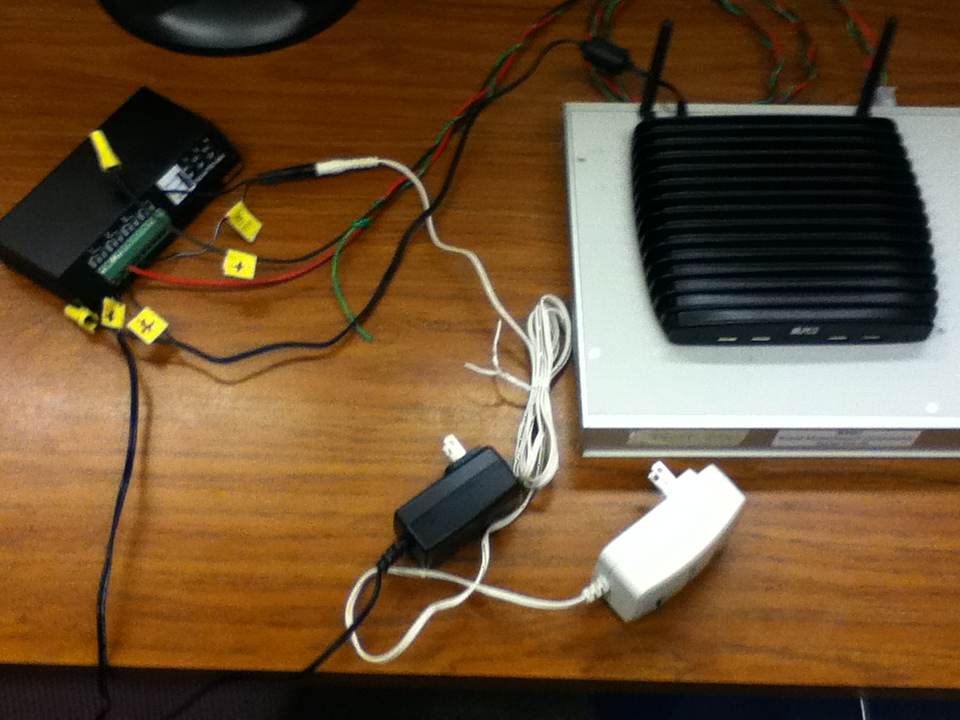
\includegraphics[scale=0.24]{pictures/power_rmg_computer.JPG}
  \end{center}
  \caption{Network powerswitch, field computer, and RMG receiver.}
  \vspace{-10pt}
\end{wrapfigure}
and processing power. The fit-PC3 suites our needs well.\footnote{For details, visit
\href{http://www.fit-pc.com}{\tt fit-pc.com}.} The fit-PC3 has a dual-core, 32-bit AMD
processor, 2 GBs of ram, and a 8GB solid state drive. Although it is designed to run 
any general-purpose desktop OS, the fit-PC3 can easily be configured to 
run as a headless system. It even comes with a mini-rs232 console interface, though 
we don't make use of this in QRAAT at the moment. With our software running full-bore, the fit-PC3 
draws 46 W. 

\textbf{Powerswitch}. The powerswitch, field computer,
and network router are connected with an ethernet switch. The field computer and RMG 
receiver are powered by a network-addressible powerswitch. The computer's power is 
switched over the network by the server, and the the computer is set up to switch the receiver. 
This makes it possible to turn the equipment on and off remotely and, with certain products, 
monitor power levels. We've deemed this feature necessary for two reasons: one, an intermittent 
issue related to the RMG receiver's USRP\footnote{For details, visit
\href{https://www.ettus.com}{\tt ettus.com}.} can be fixed by cycling the power. Remote 
switching makes fixing this problem much more convenient; two, turning off equipment, 
in particular the RMG receiver, when it's not needed is the best way to save battery power.
(Note that it is possible to deploy QRAAT without such switches.) 

Again, there are various solutions for network power switching. Most of these input 
mains power, i.e. 120 V AC, and require us to mofidy them to work with our solar 
panels (12 V DC). The PingBrother EPIW104P\footnote{For details, visit
\href{http://www.pingbrother.com}{\tt pingbrother.com}.} passive POE ethernet switch 
not only allows us to input the proper power, but provides an array of features 
uesful for our deployment of QRAAT. The EPIW104P can switch a 12 V DC relay instead of
POE, and the ethernet ports can be used as a switch. In addition, its http-based 
interface can be used to monitor the input voltage and power consumption. Our nominal 
hardware specification with the PingBrother powerswitch and fit-PC3 is as follows: 

\begin{description}
  \item[\quad Network] The network router and field computer are plugged into the 
    powerswitch's ethernet switch. The powerswitch and computer are assigned static
    IP addresses in the subnet of the router. Static addresses are necessary because 
    the QRAAT server must know how to reach the site; this information is not 
    distributed when the node comes into the network. (See software overview section 
    for details.) 
    
  \item[\quad Power] The field computer's power is attached to the powerswitch's 
    first relay on NC ("normally closed"). If power goes down and is then made 
    available the field computer will be powered automatically. The RMG receiver is
    attached to the second relay on NO ("normally opened") so that it won't get power 
    until it is needed by the computer. 
    
  \item[\quad Receiver] The receiver has a two ports: one, a straight-through serial 
    port for communication with the receiver's PIC interface, and two, a standard USB
    2.0 port for data transfer from the USRP. The fit-PC3 doesn't have a straight-through
    serial interface, but an off-the-shelf a serial $\rightarrow$ USB converter is 
    sufficient. The PIC uses a 9600,8n1 baud-rate/parity-bit scheme.  
\end{description}
 
\subsection{Software}
We begin this section with an eagle eye view of the QRAAT dataflow. Each transmitter emits 
a periodic pulse on a specific radio frequency, e.g. 164.599 Mhz. The pulse is received and
amplifed on four channels, then converted to a digital signal by the RMG receiver.
The software-defined radio filters the signal and inputs it into a pulse detector. When the 
pulse detector is triggered, the signal region surrounding the pulse on all four channels
is dumped to file. This kind of record is created for each pulse and each transmitter
that the SDR is conifgured to listen to. These files are produced and stored in memory 
on site; when the server requests them, they are tranferred over the network and deleted from
the field computer. 

The backend software package is comprised of two elements: one, the software defined radio 
module, and two, a system for managing QRAAT's resources and collecting data. We now describe 
these in turn. This section refers to the software repository published on Github at 
\href{http://github.com/QRAAT/QRAAT/}{\tt github.com/QRAAT}.

\subsubsection{RMG module}
The SDR pulse detector is implemented with a mixture of C++ and Python on top of 
GNU Radio.\footnote{\href{http://gnuradio.org/redmine/}{\tt gnuradio.org}.} 
In GNU Radio terms, the module is made up of a radio signal processing block with a suite 
of high-level applications that run it. The transmitters that the RMG module listen for
are specified by a file called \texttt{tx.csv}. (See Appendix A for file format.) When 
the software starts, a signal filter and peak detector is instantiated for each 
frequency passed by \texttt{tx.csv}, up to 32. The pulse data files are stored in a 
directory structure that reflects the time and date it was created. For example: 
\begin{verbatim}
  /tmp/ramdisk/det_files/2013/03/22/15/20/03439743.det
\end{verbatim}
The file name gives the second it was created with millisecond precision, i.e. 
\texttt{SSUUUUUU.det}.

\subsubsection{Dataflow}
Each QRAAT node has a state associated with it: \textit{down}---computer should shutdown,
\textit{up}---computer should be on, but the RMG receiver should be off and not listening 
for transmitters, or \textit{active}---the RMG receiver should be on and pulse detector should
be running. The state is specified by a file on the server called \texttt{sitelist.csv}.
(See Appendix A for file format.) Along with the state, the site list specifies the 
configuration information of each site. The parameters are:
\begin{description}
  \item \textit{Name} --- of the site, 
  \item \textit{CompIP} --- hostname or IP address of the remote computer, 
  \item \textit{PowerIP} --- hostname or IP address of the network addressible power switch,
  \item \textit{CompOutlet} --- outlet number of the computer, 
  \item \textit{RxOutlet} --- outlet number of the RMG receiver, 
  \item \textit{PowerType} --- power source type, e.g. Netbooter, PingBrother, or WebPowerSwitch, and finally
  \item \textit{State} $\in$ \{\textit{Up}, \textit{Down}, \textit{Active}\}.
\end{description}

When a site's configuration information needs to be updated or the user wishes to change 
its state, the parameters (\textit{PowerIP, RxOutlet, PowerType, State}) are transmitted to the
site computer as a configuration file called \texttt{site.csv} (Appendix A). 

\textbf{Node}. Although the node's \textit{goal} state is specified by the server, the server
cannot directly coerce its state; only the node can power on its RMG receiver and start the RMG
module or power itself down. We've designed it this way so that the nodes can function independently
of the server in case of network failure. In addition to controlling its own state, the node 
implements monitoring and error recovery by checking its state periodically. If the pulse detector
crashes for any reason, the process is controlled by a monitor script that cycles the recevier's 
power and attempts to restart the module. If the process crashes a certain number of time before 
the system successfully reaches \textit{active}, the node gives up. Each time the site's state is 
checked or transitioned, the \textit{real} state, which we'll call \textit{SiteStatus}, is 
reported to a file called \texttt{status.log}. 

\textbf{Server}. There are three essential tasks that the server implements: one, pole the 
sites for status information, two, update the sites' configuration and goal state, and three,
download and store pulse data. When a site is poled, the server collects network and site status. 
If the site is reachable, then the server reads the last line of \texttt{status.log}. Site status
is reported as (\textit{NetworkStatus, SiteStatus}). After a site is updated (the \texttt{site.csv} 
file is transmitted to the field computer), the server instructs it to check its state. 
   
Finally, when the server fetches the pulse data files, it downloads all available files excluding 
those that were recently produced (within the last minute). This is to avoid attempting to download 
a file that is currrently being written by the RMG module. Note that this design critically depends 
on real time clock synchronization, which we achieve through the \texttt{ntpd}\footnote{Network time 
protocol (NTP).} daemon. 

\subsection{Usage}
In the QRAAT protoype system, dataflow and site management are implemented with shell scripts. The
user-level programs are \texttt{rmg} and \texttt{rmg-node}. When invoked, they immediately 
set up environment variables specifying data, configuration files, etc. 

\textbf{rmg}.\footnote{The name "rmg" is admittedly a bit of a misnomer, since it 
has nothing to do with "Rapid Multichannel Goniometers". It just stuck, I suppose.} The server
control program. \texttt{rmg} takes as arguments a task and a list of sites. Before performing 
the task, the status of the site is checked. Possible tasks are the following: 
\begin{description}
  \item[\quad \textbf{status} ---] Just report site's current status as (\textit{NetworkStatus, SiteStatus}).
  \item[\quad \textbf{update} ---] Passive site update. Copy new \texttt{site.csv}. 
  \item[\quad \textbf{up/down/start/stop} ---] New goal state. Update \texttt{sitelist.csv} and copy new 
    \texttt{site.csv}. Tell the site to check its new state (\texttt{rmg-node check}, see below.) 
  \item[\quad \textbf{on/off} ---] Switch the field computer's power supply. 
  \item[\quad \textbf{updatetx --file \textit{FILE}} ---] Update site's \texttt{tx.csv}.
  \item[\quad \textbf{cyclerx} ---] Cycle the site's receiver power. This is needed sometimes. 
  \item[\quad \textbf{fetch} ---] Download \texttt{.det} files.  
\end{description}

\textbf{rmg-node}. Control a site's state locally. This program is used for monitoring 
and is invoked by \texttt{rmg} when the user changes the site's goal state. It can also be safely
called directly. As its argument, it accepts either a new state or \texttt{check}: 
\begin{description}
  \item[\quad \textbf{active} ---] Check that RMG receiver is on and the SDR is running. 
  \item[\quad \textbf{up} ---] Check that the RMG receiver is off and the SDR is stopped. 
  \item[\quad \textbf{down --delay \textit{M}} ---] Set a timer to shutdown. If such a timer 
    exists (i.e., state is already down), the timeer has elapsed and no $M$ isn't specified, than 
    power off the computer. If a delay is specified, reset timer to $M$ minutes. 
  \item[\quad \textbf{check} ---] Look up goal state in \texttt{site.csv} and transition
    as described. 
\end{description}


\section{Dataflow specifications}
QRAAT is composed of nodes all capable of running software defined radio to perform
initial signal processing. One of these is desginated as the QRAAT server, where 
pulse data are collected for higher-order processing. We've designed QRAAT with 
modularity in mind; it's possible to run the SDR on the same machine as the server. 
This dataflow is implemented as a set of shell and Python programs. Except
for the top-level \path{rmg} and \path{rmg-node} scripts, these are used by 
both the nodes and server. In this section, we describe these programs in detail. 
The complete specification of the nodes and server are also given. 



\subsection{Environment variables (\texttt{rmg\_env})}
Dataflow is implemented as a set of shell scripts and Python programs. Locations of
data, metadata, and miscellaneous variables are defined in a bash script called 
\path{rmg_env} which is included in any top level program. (See Appendix C for 
suggested values.) 

\begin{description}
  \item[\quad \path{RMG_SITE_METADATA_DIR} ---] Location of metadata on a remote 
   machine. Files included in this directory are: \path{site.csv}, \path{tx.csv}, 
   and \path{status.log}. Any debug information is also stored here. We currently 
   log the standard output and standard error of the last run of the pulse detector. 
   This value is used by the server and must be the same at each site. 

  \item[\quad \path{RMG_SITE_DET_DIR} ---] Location of data on a remote machine. 
   This is typically a subdirectory of a temporary filesystem created with 
   \path{/etc/fstab}. This value is used by the sever and must be the same at 
   each site. 
  
  \item[\quad \path{RETRY_MAX} ---] The maximum number of attempts to start the 
   pulse detector before a fatal error state is reached. This value is needed 
   by the site. 
   
  \item[\quad \path{RMG_SERVER_METADATA_DIR} ---] Location of metadata on the 
   server. Files included in this directory are \path{sitelist.csv} and transmitter
   spec files.

  \item[\quad \path{RMG_SERVER_DET_DIR} ---] Location of raw pulse data files 
   fetched from the nodes.
  
  \item[\quad \path{RMG_SERVER_EST_DIR} ---] Location of callibrated data files. 
  
  \item[\quad \path{RMG_SERVER_SSH_KEYFILE} ---] Location of private RSA encryption
   key. 
  
\end{description}


\subsection{Server} 
Along with managing the field computers and collecting data, the server is responsible for
callibration and triangulation. The \texttt{rmg} script allows us to power the computer and 
RMG module on and off, cycle the RMG module power, start and stop the software defined radio, 
update the field computer's transmitter file, and collect \texttt{.det}s. The server has a 
file called \texttt{sitelist.csv} that stores various parameters as well as the state of 
nodes. Because the server doesn't direclty control the state of the nodes, this is referred to
as the goal state. The following parameters are specified per site: 
\begin{description}
  \item \textit{Name} --- of the site, 
  \item \textit{CompIP} --- hostname or IP address of the remote computer, 
  \item \textit{PowerIP} --- hostname or IP address of the network addressible power source,
  \item \textit{CompOutlet} --- outlet number of the computer, 
  \item \textit{RxOutlet} --- outlet number of the RMG receiver module, 
  \item \textit{PowerType} --- power source type, e.g. Netbooter, PingBrother, or WebPowerSwitch, and finally
  \item \textit{State} $\in$ \{\textit{Up}, \textit{Down}, \textit{Active}\}.
\end{description}
Possible states are: 
\begin{description}
  \item \textit{Up} --- Site computer is on, the RMG receiver is off, and the pulse detector 
    is not running. 
  \item \textit{Down} --- The RMG receiver is off and either the computer is off or there 
    is a timer set on site to shutdown. The server does not directly run the shutdown the 
    on the node. 
  \item \textit{Active} --- Site computer is on, the RMG receiver is on, and the pulse detector is
    running. 
\end{description}

When a site's goal state is to be updated, the parameters (\textit{PowerIP, RxOutlet, PowerType, State})
are transmitted to the site computer in a file called \path{site.csv}. The site computer then immediately
verifies that it's actual state is \textit{State}. 

Status is reported as the pair (\textit{NetworkStatus, SiteStatus}). \textit{NetworkStatus}
is either \textit{ErrorPower}, meaning the site's powerswitch couldn't be reached over the network, 
or \textit{ErrorComputer}, meaning the powerswitch could be reached, but not the computer. If the 
computer is reachable, then \textit{NetworkStatus} = \textit{Ok}. \textit{SiteStatus} is the actual 
state reported by the site computer. If it can't be reached, then \textit{Unknown} is reported. 

To determine reachibility of the computer, the powerswitch is queried for the power status of the 
computer. If it's off, then it's assumed to be reachable if it were turned on; hence, (\textit{Ok}, \textit{Down})
is reported. If it's on and the computer is unreachable, then (\textit{ErrorComp}, \textit{Unknown}) is reported. 
Note that this status will be reported even when the field computer shuts itself down cleanly; though the system
is halted, its input is still powered and must be switched. 

\subsection{Nodes}
Field computers run the pulse detection software on GNU Radio. As such, QRAAT must be
run on GNU/Linux. Section 3 details the installation and configuration of our
software on Ubuntu Server 12.04 LTS. In addition to GNU Radio, each site must run 
an ssh daemon, git, and ntpdate. Each node has a user called \textit{rmg} who runs the SDR. 

RSA encryption is used over ssh for secure data transfer between nodes and server. The 
public key is stored on the node in \path{/home/rmg/.ssh/authorized_keys} and the private key
is stored on the server in the file specified by \path{RMG_SERVER_SSH_KEYFILE}. (See Appendix B.)

The software defined radio emits a file per pulse per transmiter and stores it 
locally in memory. To accomplish this, a temporary file system, called a ramdisk, 
is created in \path{/etc/fstab}. The location must be the parent directory 
of \path{RMG_SITE_DET_DIR}. 

Though the \textit{goal} state is specified by the server, nodes control and report their actual state 
The site computer periodically checks the goal state given in 
\path{site.csv} and verifies the computer is in that state, looks up the last reported 
status, and reports change in the real state to \path{status.log}. \textit{SiteStatus} is 
reported as one of the following: 

\begin{description}
  \item \textit{Up} --- Site computer is on, the RMG receiver is off, and the pulse detector 
    is not running. 
  \item \textit{Down(N)} --- Site computer is on, the RMG receiver is off, the pulse detector is 
    on, and a timer is set to power down the system. If $N$ seconds have elapsed since the 
    site last checked its status, then \textit{Shutdown} is reported and computer powers itself
    off. 
  \item \textit{Shutdown} --- If this is the last reported status and the goal state is \textit{Down}, 
    then the shutdown timer is reset. 
  \item \textit{Active} --- Site computer is on, the RMG receiver is on, and the pulse detector is
    running 
  \item \textit{ErrorRetry(i)} --- The pulse detector crashed and is restarting. The software 
    may crash for various reasons, sometimes resulting from upstream code such as GNU Radio
    or the driver for the USRP. Before retrying, the RMG receiver's power is cycled. $i$ gives
    the retry count. 
  \item \textit{ErrorFatal} --- $i$ = \path{RETRY_MAX}, do not attempt to recover. The computer
    remains on, but the RMG receiver is off. 
\end{description}


\subsection{Programs}
\subsubsection{\texttt{rmg\_csv}}
\begin{verbatim}
    usage: rmg_csv <site> <parameter> [<value>] 
              -c,--column <parameter> [<value>] 
              -r,--row <site> [{parameter list}]
              -l,--last-row   [{parameter list}]
     < path/to/original.csv [> path/to/new.csv]
\end{verbatim}
This program is used to look up and modify values in configuration files. It's functionality
has evolved to meet our needs. The input is a CSV-formatted file on standard input. If a 
the name of a site and a paramter are given as arguments, then \path{rmg_csv} emits that 
field. If the field is empty, it emits \textit{nil}. If a value is also passed, then 
the CSV file is dumped to standard output with 
the field replaced. The '\texttt{-c}' option is similar, but it's applied to each site (row). 
The '\texttt{-r}' option emits a row as a CSV file. If a parameter list is given, then 
the fields for the row are outputted on separate lines. '\texttt{-l}' has a similar 
functionaility, but it applies to the last row. This is uesful for polling site status
from \path{status.log}.


\subsubsection{\texttt{rmg\_fetch}}
\begin{verbatim}
    usage: find <dir> -type d | rmg_fetch 
\end{verbatim}
\path{rmg_fetch} is used to compile a list of directories of pulse data files to fetch
from a remote computer. \path{scp} is used to copy whole directories from the nodes 
to the server. Recall that data files are stored in a directory structure 
based on the date and time they were created. In order to prevent copying a file currently 
being written by the pulse detector, we exclude directories created within the 
last minute. Thus, if the current time is 15:20 on 22 March 2013, we can't simply 
the entire directory \path{/tmp/ramdisk/det_files/2013}; we have to copy all the sibling
directories of \path{/tmp/ramdisk/det_files/2013/03/22/15/20} individually. \path{rmg_fetch}
combines non-"hot" directories in order to reduce the number of calls to \path{scp}. It reads
a directory structure on standard input and outputs a list of subdirectories that can be 
copied at once. 
  
  
\subsubsection{\texttt{rmg\_powerswitch}}
\begin{verbatim}
    usage: rmg_powerswitch <pwr_type> <pwr_ip> <outlet> {ON, OFF, CYCLE, QUERY} 
                           [--invert={true,false}]
\end{verbatim}
We use this script to control network addressible powerswitches. \path{pwr_type} $
\in$ \{\textit{pingbrother}, \textit{webpowerswitch}, \textit{netbooter}, \textit{nil}\} is the 
type (brand) of powerswitch, \path{pwr_ip} is its address, and \path{outlet} is 
the identifier (number) of the outlet to be switched. \path{QUERY} returns the status of the 
outlet specified, either 1 or 0. If the '\path{--invert}' option is passed, then 
\textit{ON} is sent to the relay instead of \textit{OFF} and vise-versa. This feature is 
useful for the PingBrother system when a device is attached to NO instead of NC. 


\subsubsection{\texttt{rmg\_runretry}}
\begin{verbatim}
    usage: rmg_runretry <pwr_type> <pwr_ip> <rx_outlet>
\end{verbatim}
\path{rmg_runretry} is a wrapper script for the pulse detector and as such is only
run on nodes. It starts the pulse detector and waits for it to fail. Once it fails, 
it cycles the power of the RMG receiver with \path{rmg_powerswitch} and retries up 
to \path{RETRY_MAX} times. After each failure, the status is written to \path{status.log}
with the retry count. After \path{RETRY_MAX} failures, \textit{ErrorFatal} is reproted and 
the program closes. Because this script is normally called from a higher level
program, \path{RETRY_MAX} is expected to be declared before runnning.

\subsubsection{\texttt{rmg-node}}
\begin{verbatim}
    usage: rmg-node state/check [-options]
\end{verbatim}
(Detailed usage in overview section.) \path{rmg-node} is used to change the state 
of a QRAAT node locally. Either the state is specified or \textit{check} is given and the
program verifies the real state is consistent with the goal state specified in 
\path{RMG_SITE_METADATA_DIR/site.csv}. First, the script loads \path{rmg_csv} and 
verifies that configuration information is available. If no \path{status.log} exists, 
one is created. Next, current status information is collected, including the RMG 
receiver power state, the process I.D. of the pulse detector (if it's running), and
the timestamp of the last-known status. We set up each node with the cron task 
\texttt{rmg-node check}.

\subsubsection{\texttt{rmg}}
\begin{verbatim}
    usage: rmg task [-options] {site list}/all 
\end{verbatim}
(Detailed usage in overview section.) \path{rmg} is used to monitor and manipulate the 
state of QRAAT. Before \textit{task} is performed, the status of the site is checked, 
i.e. (\textit{NetworkStatus, SiteStatus}) is reported. If the task is only to report 
the status, a warning is emitted if the site's goal state is not consistent with the
server-specified goal state. When an update or state-transition is to be performed, 
the server transmits the relevant \path{site.csv} to the field computer and runs 
\texttt{rmg-node check}. 

\path{rmg} is also capable of some other miscellaneous tasks that don't cause state 
checks. These are \path{cyclerx}, which cycles the RMG receiver's power directly 
from the server, and \path{updatetx}, which transmits a new transmitter file to 
the site. Note that \path{updatetx} doesn't cause a running pulse detector to reload its 
tranmitter configuration. 


\section{Configuration instructions}

\subsection{Field computers}
The field computers were configured by building and installing the software on one 
system, creating an image from its harddrive, and copying this image to the other sites. To create
the image, we first installed a stock copy of Ubuntu Server 12.04 on a 7.5 GB partition, leaving
512 MB for swap. We configured no automatic updates, since these computers spend the majority of 
their time not connected to the internet. After booting the system and updating, the first thing
to do is install the following packages via apt-get: 
\begin{enumerate}
  \item \texttt{git-core} - clone our software repository from github.
  \item \texttt{openssh-server} - each field site needs to run an ssh daemon.
  \item \texttt{minicom} - serial interface to RMG receiver module.
  \item \texttt{ntpdate} - remote computers will be clock synced to the server via \texttt{ntpd}. 
\end{enumerate}

\subsubsection{Building and installing the software}
Clone the online repository to get things going:
\begin{verbatim}
$ git clone github.com/QRAAT/QRAAT.git
\end{verbatim}
The first thing to build is GNU Radio along with the UHD driver. For conveniance, we provide a copy 
of the gnuradio build script written by Marcus Leech. Type
\begin{verbatim}
$ QRAAT/build-gnuradio -v all
\end{verbatim}
to start downloading and building. This may take a few hours, but you'll only need to do this once. When the 
build finishes, it will output a couple post-install tasks. Make sure you do these. Next, building
and installing the QRAAT software is essentially the same procedure, though it will take less than 
two minutes: 
\begin{verbatim}
$ QRAAT/build-rmg -v install
\end{verbatim}

To handle updates in this early development stage, we've set up each node to clone 
the software repository from the QRAAT server. The code base is stored locally in
\path{/home/rmg/QRAAT}. To update, ssh to the site, switch to this directory, and type
'git pull'.

Before testing your build, we need to setup communication with the RMG recevier's PIC interface. First we 
add a rule to udev\footnote{\texttt{udev} is a common domain on GNU/linux systems used to handle 
new devices when they're plugged in. For instance, when you installed GNU Radio, rules were installed 
for the USRP---a hardware component of the RMG receiver---and the UHD driver.} to set permissions for 
\texttt{/dev/ttyUSB0}, the serial interface for the RMG receiver. Create a new file: 
\begin{verbatim}
$ sudo vi /etc/udev/rules.d/101-serial-usb.rules
\end{verbatim}
and type the following line: 
\begin{verbatim}
  KERNEL=="ttyUSB0", MODE="0666"
\end{verbatim}
To verify that this worked, we'll try to communicate with the PIC via minicom. Open up the minicom
configuration screen. Under \textit{Serial port setup}, set \textit{Serial Device} to \texttt{/dev/ttyUSB0}.
Set \textit{Bps/Par/Bits} to \texttt{9600 8N1}. Lastly, set \textit{Hardware/Software Flow Control} to 
\texttt{No}. Restart minicom. See if you're able to communicate with it by typing "\texttt{?}".  

\subsubsection{Post-configuration} 

The SDR pulse detetcor can potentially produce a lot of files, and since they aren't needed 
permanently down stream, we store them locally in memory. We create a temporary file system 
in RAM in order to accomplish this. Add the following line to the end of \texttt{/etc/fstab} (be careful!): 
\begin{verbatim}
tmpfs   /tmp/ramdisk  tmpfs  nodev,nosuid,mode=1777,size=1024M   0   0
\end{verbatim}
1 GB is reasonable since the field computers have 2 GBs of ram. 

If linux shuts down uncleanly, e.g. the site loses power, the GRUB bootloader will wait for user 
input before rebooting the operating system. This is bad for headless systems, so we need to 
configure GRUB to timeout in this situation. Add the following to /etc/default/grub: 
\begin{verbatim}
  GRUB_RECORDFAIL_TIMEOUT=2
\end{verbatim}
Then type \texttt{sudo update-grub}. 

Up until now, we've been using the field computer with a monitor, keyboard, and ethernet connection
to the internet. The next thing we have to do is configure the network interface so that we can 
access it over ssh without a head. In \path{/etc/network/interfaces}, comment out the default 
ethernet interface and add a static IP address: 
\begin{verbatim}
  # auto eth0
  # iface eth0 inet dhcp
  auto eth0
  iface eth0 inet static
    address 10.20.1.55
    netmask 255.0.0.0
\end{verbatim}
To connect to the computer directly through an ethernet cable, just setup a static IP address on 
the host system in the same subnet. See the section on networking for details. 

The next thing to do is change the system's hostname. This needs to be changed in two places:
\path{/etc/hostname} and \path{/etc/hosts}. 

Lastly, since we will be managing the power of this system remotely, we want to be able to 
shutdown and reboot the computer without typing in a sudo password. Type 
\begin{verbatim}
$ sudo visudo
\end{verbatim}
and add the following lines to the end of the sudoers file: 
\begin{verbatim}
  rmg ALL=NOPASSWD: /sbin/halt
  rmg ALL=NOPASSWD: /sbin/reboot
  rmg ALL=NOPASSWD: /sbin/poweroff
\end{verbatim}

\subsubsection{Creating an image}
The preceeding configuration is time-consuming, though not difficult. For configuring many sites, 
it's best to create an image from a fully configured system and copy this to other sites. The 
simplest way to do this is with an Ubuntu live-USB. Plug a monitor, keyboard, and mouse into the 
FitPC and boot a live copy of Ubuntu on a thumbdrive. Grab a terminal and make sure the harddrive
is unmounted. ("\texttt{mount | grep sda}"). Verify that /dev/sda is indeed the 
harddrive.) Plug in an external harddrive or thumbdrive that can 
fit the 8 GB file we're about to create. Change the directory to the external drive and run: 
\begin{verbatim}
$ dd if=/dev/sda of=qraat.img bs=4K 
\end{verbatim}
To copy the image, boot another computer in the same way. Plug in the external drive, change to 
its directory, and type
\begin{verbatim}
$ dd if=qraat.img of=/dev/sda bs=4K
\end{verbatim}

Both of these commands should take about 30 minutes. Once you've finished copying the image, you'll 
want to edit the hostname and network interfaces as described in the preceeding section. 



\subsection{Networking}
These instructions apply to our deployment at Quail Ridge. 
The ethernet interface needs to be configured to use the Qurinet router as its gateway. 
In /etc/network/interfaces, you'll find an interface that is commented out. 
Uncomment this and comment out the old one. 
\begin{verbatim}
  # Default interface in Quirinet
  auto eth0 
  iface eth0 inet static
    address 10.20.1.55
    netmask 255.255.0.0
    gateway 10.20.1.1
\end{verbatim}

The second part is to make sure the git repository is pointed to the right place. In 
/home/rmg/QRAAT/.git/config, you'll find a line that reads
\begin{verbatim}
  url = christopher@10.253.1.55:work/QRAAT # change me!
\end{verbatim}
Change this to the correct user and directory and you're set!

\pagebreak
\begin{appendices}

\section{Configuration files}
QRAAT metadata is stored in CSV-style files. Elements are seperated by commas and 
spaces are not allowed. The first row specifies the column parameters. Values may
be ommited. 

\textbf{tx.csv}. The transmitter file maps a name to frequency and also passes 
parameters to the pulse detector. These are described in detail in the backend
software manual. 
\begin{verbatim}
use,name,freq,type,pulse_width,rise_trigger,fall_trigger,filter_alpha
yes,robin1,164.42,Pulse,20,3.0,2.0,0.01
yes,robin1_heart,164.65,Continuous,,,,
no,noisy,164.5,Pulse,20,1.010,1.005,0.01
yes,test_tx,165.99,Pulse,25,3.00,1.15,.001
yes,mouse1,164.3,Pulse,25,3.0,2.0,0.01
\end{verbatim}

\textbf{sitelist.csv}. The site list stores information about the nodes that is needed
by the server. 
\begin{verbatim}
name,comp_ip,power_ip,comp_outlet,rx_outlet,powertype,state
site0,10.0.0.55,10.0.0.56,1,2,webpowerswitch,down
site1,localhost,,,,,up
site2,10.2.1.55,10.2.1.56,1,2,netbooter,up
site10,10.10.1.55,10.10.1.56,2,3,pingbrother,up
site13,10.13.1.55,10.13.1.56,1,2,pingbrother,active
site20,10.20.1.55,10.20.1.56,1,2,pingbrother,down
site21,10.20.1.55,10.21.1.56,1,2,pingbrother,active
\end{verbatim}

\textbf{site.csv}. Each field computer has a file that specifies its own configuration. 
This is necessary so that it can switch the receiver's power, as well as check its own 
goal state. 
\begin{verbatim}
power_ip,rx_outlet,powertype,state
10.13.1.56,2,pingbrother,active
\end{verbatim}

\textbf{status.log}. Each field computer keeps a log as a time stamp
in seconds since the epoch and its status when checked. 
\begin{verbatim}
timestamp,site_status
\end{verbatim}
\quad \quad $\cdots$
\begin{verbatim}
1366307941,up
1366312980,active
1366312996,up
1366313467,down(300)
1366313445,shutdown
1366323435,down(300)
1366323974,up
\end{verbatim}

\section{Creating an encryption key}
We use RSA encryption for communication between server and nodes for secure transmission
as well as efficient SSH scripting, since RSA keys don't require a password. 
Here's how we made a key.

On the server:\\
\texttt{\$ ssh-keygen -t rsa}\\
\texttt{Generating public/private rsa key pair.}\\
\texttt{Enter file in which to save the key (/home/christopher/.ssh/id\_rsa):} [type "rmg\_rsa"]\\
\texttt{Enter passphrase (empty for no passphrase):} [press enter]\\
\texttt{Enter same passphrase again:} [press enter]\\
   ... some output ... \\
\texttt{\$ mv rmg\_rsa ~/.ssh/rmg\_rsa}\\
\texttt{\$ scp rmg\_rsa.pub rmg@site}$N$\texttt{:rmg\_rsa.pub}\\
\texttt{\$ ssh rmg@site}$N$\\

On remote site $N$:\\
\texttt{\$ mkdir -p .ssh \&\& mv rmg\_rsa.pub .ssh}\\
\texttt{\$ cat .ssh/rmg\_rsa.pub >> .ssh/authorized\_keys}\\

Test setup (on RMG Server):\\
\texttt{\$ ssh -i .ssh/rmg\_rsa rmg@site}$N$\\
\texttt{\$ rmg fetch site}$N$\\

\section{Suggested environment variable values}
QRAAT's variables are defined in \path{rmg_env} and are included at the start of both 
\path{rmg} and \path{rmg-node}. The default values for these variables are given as 
follows: 

\begin{verbatim}
RMG_SITE_METADATA_DIR="/home/rmg"
RMG_SITE_DET_DIR="/tmp/ramdisk/det_files"
RETRY_MAX=10
RMG_SERVER_SSH_KEYFILE="$HOME/.ssh/rmg_rsa"
RMG_SERVER_DET_DIR="$HOME/det_files"
RMG_SERVER_EST_DIR="$HOME/est_files"
RMG_SERVER_METADATA_DIR="$HOME"
\end{verbatim}

\end{appendices}

\end{document}
